\chapter{Studio fattibilità app in \textit{monorepo}}
\label{chap:studio_fattibilita}
\section{Cos'è una \textit{monorepo}}
Una \gls{monorepog}\glox è un singolo \gls{repog} che contiene più progetti, spesso correlati.
Questo approccio consente di mantenere tutto il codice sorgente in un'unica posizione, facilitando la condivisione di codice e la gestione delle dipendenze.
Una \textit{monorepo} può contenere applicazioni \gls{frontendg}\glox e \gls{backendg}\glox, librerie condivise e altre risorse comuni, permettendo una gestione centralizzata del progetto.
A differenza di un semplice \textit{code colocation}, dove diversi progetti sono collocati nello stesso \textit{repository} senza relazioni definite, una \textit{monorepo} promuove l'integrazione e la gestione coesa dei progetti.
Le relazioni ben definite tra i progetti all'interno di una \textit{monorepo} permettono una modularità e una divisione del codice che ne facilitano la manutenzione e lo sviluppo.
Contrariamente alla percezione comune, una buona \textit{monorepo} è modulare e non monolitica.
La modularità permette di mantenere la separazione delle preoccupazioni e facilita il riutilizzo del codice tra i diversi progetti.
Una \textit{monorepo} ben strutturata si oppone all'idea di un \textit{monolite}, che invece rappresenta un grande blocco di codice non suddiviso in parti discrete.
Per contrasto, un \textit{multirepo} è l'approccio standard attuale per lo sviluppo delle applicazioni, dove ogni \textit{team}, applicazione o progetto ha il proprio \textit{repository}.
Questo metodo permette autonomia ai \textit{team} nello scegliere le librerie, nei tempi di \textit{deploy} delle applicazioni e su chi può contribuire al codice.
Tuttavia, questa autonomia è ottenuta tramite l'isolamento, che può danneggiare la collaborazione e creare vari problemi di gestione delle dipendenze e di integrazione.
Utilizzare una \textit{monorepo}, quindi, offre il vantaggio di una maggiore integrazione e collaborazione tra i \textit{team}, pur mantenendo la modularità e la divisione del codice necessarie per una gestione efficace e scalabile del progetto.

\begin{figure}[H]
\centering
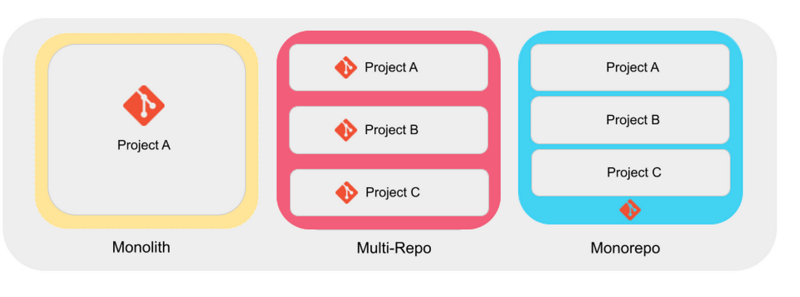
\includegraphics[alt={Differenze tra \textit{monolith multi-repo e monorepo}}, height=5cm]{img/monorepocompare.png}
\caption{\textit{Monolith vs Multirepo vs Monorepo}}
\label{fig
}
\end{figure}

\pagebreak

\section{Gestione delle dipendenze}
Una \textit{monorepo} può avere strutture diverse e una differenza fondamentale la fa la gestione delle dipendenze. 
All'interno dei progetti \textit{JavaScript}, un primo approccio per creare il proprio progetto in \textit{monorepo} potrebbe essere utilizzando \textit{NPM Workspaces}.
Nel progetto di Stage \textit{DDC Service}, questo è stato introdotto in questa maniera.
Utilizzare \textit{NPM Workspaces} è un approccio molto semplice che non richiede modifiche strutturali importanti alla \textit{codebase}; tuttavia, è adatto per progetti con una complessità inferiore.
Finché si hanno due applicazioni e due o tre librerie condivise, questa struttura potrebbe andare bene, ma quando si introducono gradi di complessità maggiori, come nel caso di \textit{DDC Service}, questo approccio non è facilmente utilizzabile.
Già arrivando a un grado di complessità come l'attuale struttura della \textit{monorepo} con quattro app e cinque \textit{packages}, la \textit{monorepo} non è scalabile e manutenibile.
La differenza la fa la gestione delle dipendenze.
Con gestione delle dipendenze non si intende solo quali pacchetti esterni si ha bisogno, ma soprattutto di quale versione.

\pagebreak
\subsection{Gestione delle dipendenze decentralizzata}
L'approccio con \textit{NPM Workspaces} utilizza una struttura decentralizzata per la gestione delle dipendenze, delegando a ciascun progetto il compito di definire le proprie dipendenze nel proprio file \texttt{package.json}.
Questo approccio decentralizzato può portare a diversi problemi.

Per illustrare meglio questa struttura, possiamo fare riferimento al seguente albero gerarchico che descrive la struttura di una \textit{monorepo} ipotetica:

\dirtree{%
.1 /.
.2 package.json.
.2 node\_modules.
.2 apps.
.3 A.
.4 package.json.
.4 node\_modules.
.3 B.
.4 package.json.
.4 node\_modules.
.3 C.
.4 package.json.
.4 node\_modules.
.2 packages.
.3 P1.
.4 package.json.
.4 node\_modules.
.3 P2.
.4 package.json.
.4 node\_modules.
}


\subsection{Problemi nella gestione delle dipendenze decentralizzata}

Nella struttura sopra illustrata, vediamo che ogni applicazione e pacchetto ha il proprio file \texttt{package.json} per gestire le dipendenze.
Questo può portare a diversi problemi:

\begin{itemize}
    \item \textbf{Conflitti di Versione}: Diverse versioni della stessa libreria possono causare errori difficili da diagnosticare e risolvere.
    Per esempio, se l'applicazione A richiede \texttt{dependencyZ@1.0.0} e l'applicazione C richiede \texttt{dependencyZ@2.0.0}, gestire queste versioni diverse può essere complicato e potrebbe portare a errori durante l'esecuzione.
    \item \textbf{Duplicazione di Codice}: Gestire dipendenze simili in più file \texttt{package.json} può portare a duplicazione di codice e aumento delle dimensioni del repository.
    Ad esempio, se l'applicazione A e B hanno la stessa dipendenza esterna come \texttt{dependencyX@1.0.0}, devono dichiararla in modo ridondante in ciascun loro file \texttt{package.json}.
    Questo aumento della duplicazione potrebbe introdurre inconsistenze nel tempo e richiede un aggiornamento manuale in ciascuna dichiarazione quando si desidera effettuare un aggiornamento della dipendenza.
    \item \textbf{Difficoltà di Manutenzione}: Aggiornare le dipendenze in una \textit{monorepo} decentralizzata può richiedere aggiornamenti manuali in molti file, aumentando il rischio di errori.
    \item \textbf{Funzionamento improprio di NPM}: Un problema comune è quando una dipendenza viene installata nel posto sbagliato. Se una dipendenza è installata nel posto sbagliato, potrebbe non essere rilevato immediatamente e le applicazioni potrebbero funzionare senza segnalare problemi.
    Il file \texttt{package.lock.json} di NPM memorizza le informazioni sulla \textit{dependency tree} e le posizioni delle dipendenze all'interno della cartella \texttt{node\_modules}.
    \\Ad esempio, se \texttt{dependencyX@1.0.0} è installata accidentalmente nell'applicazione B invece che in A, l'applicazione A potrebbe ancora accedere a \texttt{dependencyX} attraverso il percorso di B, rendendo difficile la rilevazione di errori.
    Consideriamo ora un caso ipotetico più complicato: se si vuole installare \texttt{dependencyY@2.0.0} come dipendenza di B, ma \texttt{dependencyY@2.0.0} richiede \texttt{dependencyX@2.0.0} come dipendenza, ci sarebbe un conflitto con \texttt{dependencyX@1.0.0} già presente in B. Sovrascrivere \texttt{dependencyX@1.0.0} con \texttt{dependencyX@2.0.0} potrebbe risolvere il problema per B, ma potrebbe rendere A incompatibile con la nuova versione di \texttt{dependencyX}.
\end{itemize}


\subsection{Problema delle peer dependencies}

Un problema comune nelle \textit{monorepo} decentralizzate sono le \textit{peer dependencies}. 
Le \textit{peer dependencies} sono dipendenze che devono essere installate esternamente al modulo che le richiede, ma devono essere presenti per evitare errori di \textit{runtime}.
Consideriamo un caso dove l'applicazione A richiede \texttt{dependencyZ@1.0.0}, che a sua volta richiede \texttt{dependencyY@1.5.0} come peer dependency.
Nel frattempo, l'applicazione B richiede \texttt{dependencyZ@2.0.0}, che richiede \texttt{dependencyY@2.0.0} come \textit{peer dependency}.
Se entrambe le applicazioni sono nella stessa \textit{monorepo} decentralizzata e ciascuna gestisce le proprie dipendenze, potrebbero installare versioni incompatibili di \texttt{dependencyY}, causando errori durante l'esecuzione o comportamenti imprevisti.
Questi problemi evidenziano le difficoltà di mantenere la coerenza e la compatibilità delle dipendenze in una \textit{monorepo} decentralizzata, spesso rendendo necessarie soluzioni più centralizzate per gestire con efficacia progetti complessi e scalabili.

\subsection{Problemi nella Gestione delle Dipendenze di DDC Service}
Nel momento in cui si è sviluppata \gls{ddcg}\glox non si sono tenute in considerazione le problematiche descritte nella gestione delle dipendenze decentralizzate.
Nel momento in cui si è iniziato lo sviluppo di \gls{ddcserviceg}\glox, nelle prime settimane di sviluppo ci sono stati diversi problemi difficilmente individuabili.
Ci sono stati alcuni momenti in cui durante l'installazione di moduli per \textit{DDC Service} questo rendeva inutilizzabile \textit{DDC}.
Per poter portare avanti lo sviluppo queste problematiche non sono state considerate e lo sviluppo ha continuato su due \textit{branch} separati.
Nel momento in cui si è voluto fare il \textit{merge} dei due \textit{branch} queste problematiche sono venute di nuovo a galla.
Sono stati evidenziati tutti i problemi descritti nella sezione superiore, come per esempio le dipendenze di \textit{DDC} non fossero fin dall'inizio installate nel posto giusto.
Si è visto come aumentando la complessità della \textit{monorepo} di solo 2X questo ha completamente reso la \textit{repository} inutilizzabile.
Queste problematiche non sono solo colpa della mala gestione dei programmatori ma sono evidenziate dalle lacune tecniche che \textit{NPM Workspaces} ha.
Quando si inizia un nuovo progetto si è tentati di iniziare utilizzando questo strumento per definire una \textit{monorepo}, tuttavia potrebbe essere una scelta sbagliata in quanto rende il progetto non estensibile in futuro.

\subsection{Benefici della Gestione Centralizzata}
Adottare una gestione centralizzata delle dipendenze offre numerosi vantaggi che risolvono i problemi tipici della gestione decentralizzata:

\begin{itemize}
    \item \textbf{Consistenza}: Tutte le parti del progetto utilizzano le stesse versioni delle dipendenze, riducendo i conflitti.
    In una gestione decentralizzata, le diverse versioni delle stesse librerie possono causare errori difficili da diagnosticare e risolvere.
    La gestione centralizzata elimina questi conflitti mantenendo una versione uniforme delle dipendenze in tutto il progetto.
    \item \textbf{Semplificazione della Manutenzione}: Aggiornare una dipendenza richiede un'unica modifica, facilitando il mantenimento del progetto.
    Con la gestione decentralizzata, ogni progetto deve aggiornare le proprie dipendenze singolarmente, aumentando il rischio di errori e la complessità della manutenzione.
    La gestione centralizzata permette di aggiornare le dipendenze in un unico punto, riducendo il rischio di inconsistenze.
    \item \textbf{Riduzione della Duplicazione}: Con un unico file \texttt{package.json}, si evita la duplicazione di dipendenze in tutto il \textit{repository}.
    La gestione decentralizzata può portare a duplicazioni di codice, aumentando le dimensioni del \textit{repository} e complicando gli aggiornamenti.
    La gestione centralizzata riduce la duplicazione, rendendo il progetto più snello e facile da gestire.
\end{itemize}

\section{Gestione delle \textit{Monorepo} con \textit{Nx}}
\textit{Nx} è uno strumento avanzato per la gestione delle \textit{monorepo} che supporta la gestione centralizzata delle dipendenze.
Utilizzando \textit{Nx}, è possibile garantire che tutte le dipendenze siano allineate, migliorando la consistenza e semplificando la gestione del progetto.
Questo strumento offre soluzioni per i problemi comuni nella gestione decentralizzata, come i conflitti di versione, la duplicazione del codice e la manutenzione complessa.

\section{Benefici di Nx}
I principali benefici di utilizzare \textit{Nx} includono:

\begin{itemize}
    \item \textbf{Aggiornamenti Globali delle Dipendenze}: \textit{Nx} obbliga l'aggiornamento delle dipendenze globalmente per l'intero progetto, migliorando la coerenza.
    In una gestione decentralizzata, aggiornare le dipendenze in modo uniforme è difficile e può portare a conflitti.
    \textit{Nx} assicura che tutte le parti del progetto utilizzino le stesse versioni delle dipendenze, eliminando questi problemi.
    \item \textbf{CI/CD Migliorato}: Una gestione centralizzata delle dipendenze facilita l'integrazione continua (CI) e la distribuzione continua (CD), riducendo i rischi di errore.
    Nella gestione decentralizzata, la \gls{cicdg}\glox può essere compromessa da dipendenze incoerenti tra i progetti.
    \textit{Nx} garantisce che tutte le dipendenze siano coerenti, migliorando la stabilità e l'affidabilità dei processi \textit{CI/CD}.
    \item \textbf{Strumenti di Sviluppo Avanzati}: \textit{Nx} offre strumenti potenti per la gestione delle \textit{build}, dei test e delle dipendenze, migliorando l'efficienza dello sviluppo.
    Questi strumenti aiutano a gestire la complessità delle \textit{monorepo}, facilitando la \textit{build} e il \textit{testing} delle diverse parti del progetto.
    Nella gestione decentralizzata, questi processi possono essere disorganizzati e inefficienti.
    \textit{Nx} centralizza e ottimizza questi processi, migliorando la produttività del \textit{team} di sviluppo.
\end{itemize}

\section{Necessità di Test Approfonditi}
In una \textit{monorepo} con gestione centralizzata delle dipendenze, è essenziale implementare test di unità, di integrazione e \gls{e2e} per garantire che ogni modifica sostanziale non comprometta l'intero progetto.
Dato che le dipendenze sono condivise tra tutti i progetti, una modifica in una dipendenza può avere effetti a catena su tutto il sistema, rendendo i test critici per mantenere la stabilità e la funzionalità della \textit{monorepo}.
Questo aiuterebbe nelle \textit{CI/CD} ma è necessario utilizzare test di unità o di integrazione.
I classici problemi che possono verificarsi durante l'installazione o l'aggiornamento di una dipendenza sono quando un altro progetto diventa non funzionante.
Per proteggersi da questo, si dovrebbe almeno testare che con ciascuna modifica gli altri progetti continuino a compilare il loro codice e ad eseguire correttamente.

\newpage